\documentclass[../../main.tex]{subfiles}

\graphicspath{{\subfix{../../immagini/}}}

\begin{document}

Un \textit{Filtro di Bloom} (\cite{Bloom1970SpacetimeTI}) è una struttura dati probabilistica basata su funzioni di hash, l'obiettivo della struttura è rappresentare un insieme di elementi in un modo tale da permettere di verificare l'appartenenza o meno di altri elementi a tale insieme. Proprietà fondamentale di un filtro di Bloom è il fatto di poter generare falsi positivi, ma non falsi negativi.

Questa struttura trova il suo principale utilizzo nei contesti in cui mantenere tutto l'insieme in memoria richiederebbe molto più spazio di quello a disposizione: il filtro infatti consiste semplicemente in un array di $n$ elementi, inizializzati a $0$, ed una serie di $k$ funzioni di hash, che mappano in modo uniforme sulle $n$ possibili posizioni. Ogni elemento appartenente all'insieme viene passato attraverso le $k$ funzioni ed i bit presenti nelle posizioni corrispondenti ai risultati vengono posti ad 1. Intuitivamente, fissata una dimensione del filtro, maggiori sono gli elementi da inserire, maggiore è la probabilità di ottenere falsi positivi.

Formalmente quindi un Filtro di Bloom è formato da:
    \begin{itemize}
        \item un array di $n$ bit, inizializzati a 0,
        \item un insieme di $k$ funzioni di hash $h_1, h_2, \dots, h_k$, tutte restituiscono, con probabilità uniforme, una posizione tra $0$ ed $n-1$,
        \item un insieme $\mathcal{S}$ di chiavi da inserire nel filtro con $|\mathcal{S}| = m$.
    \end{itemize}
Per testare l'appartenenza di un elemento $x$ al filtro è quindi necessario controllare che tutti i bit nelle posizioni equivalenti ai risultati delle funzioni di hash $h_1(x), \dots h_k(x)$ abbiano valore 1. Ovviamente quindi, data la natura delle funzioni di hash, saranno presenti delle collisioni: più elementi verranno mappati alla stessa posizione, per questo motivo se, dato $x$, una delle funzioni ritorna 0 posso essere certo della sua non appartenenza al filtro, viceversa se tutte le funzioni ritornano 1 è comunque possibile che l'elemento non appartenga all'insieme $\mathcal{S}$.

Nella figura \ref{fig:BFExample} viene mostrato l'esempio di un filtro di Bloom subito dopo la sua creazione (figura \ref{fig:BFCreazione}), subito dopo l'inserimento di tutti gli elementi in $\mathcal{S}$ (figura \ref{fig:BF:Inizializzazione}) e dell'operazione di controllo dell'appartenenza (figura \ref{fig:BFAppartenenza}).

\begin{figure}[H]
    \centering
    \begin{subfigure}[b]{0.70\textwidth}
       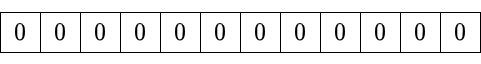
\includegraphics[width=1\linewidth]{immagini/3/bloomFilterInitial .png}
       \caption{Rappresentazione di un filtro di Bloom subito dopo la sua creazione, in questo caso il filtro ha grandezza $n = 12$, $k = 2$ funzioni di hash e deve contenere $m = 3$ elementi.}
       \label{fig:BFCreazione} 
    \end{subfigure}
    
    \begin{subfigure}[b]{0.70\textwidth}
       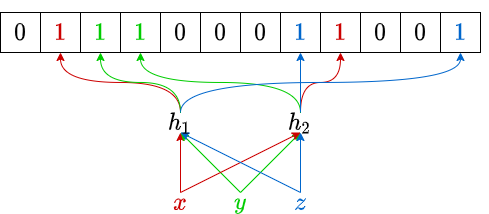
\includegraphics[width=1\linewidth]{immagini/3/bloomFilterInserimento.png}
       \caption{Rappresentazione del filtro subito dopo l'operazione di inserimento di tutti gli elementi in $\mathcal{S}$.}
       \label{fig:BF:Inizializzazione}
    \end{subfigure}
 
    \begin{subfigure}[b]{0.70\textwidth}
        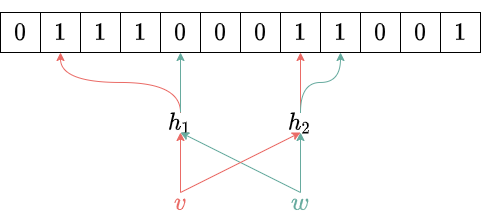
\includegraphics[width=1\linewidth]{immagini/3/bloomFilterCheck.png}
        \caption{Rappresentazione dell'operazione di controllo dell'appartenenza al filtro, nell'immagine $v$ e $w$ non appartengono all'insieme $S$. Noto come $w$ venga giustamente respinto, mentre $v$ venga accettato come elemento del filtro, generando un falso positivo.}
        \label{fig:BFAppartenenza}
     \end{subfigure}
    \caption{}
    \label{fig:BFExample}
\end{figure}

\subsubsection{Probabilità di un falso positivo}
La probabilità di ottenere un falso positivo $f$ può essere quantificata dalla formula
\begin{equation}
    f = \left(1 - \left(1 - \frac{1}{n}\right)^{km}\right)^k \approx \left(1 - e^{-km/n}\right)^k,
    \label{eqn:bloomfpr}
\end{equation}
abbiamo infatti supposto che ogni funzioni di hash mappi con probabilità uniforme su ognuno degli $n$ bit  dell'array, di conseguenza dato un elemento $x$ da inserire nel filtro, la probabilità che uno specifico bit non venga impostato a 1 dopo che l'elemento è passato per tutte le $k$ funzioni di hash è:
\[\left(1 - \frac{1}{n}\right)^k,\]
l'inserimento deve essere effettuato per tutti gli $m \in \mathcal{S}$ elementi, supponendo ogni inserimento come un evento indipendente\footnote{Nella realtà l'indipendenza tra successivi inserimenti non vale: il fatto che un bit venga posto ad 1 influenza la probabilità degli altri bit di essere posti ad uno, di fatto quindi $e^{-km/n}$ rappresenta il valore atteso della frazione di bit a 0 dopo l'inserimento, in \cite{10.1145/383962.384004} viene però dimostrato che il valore reale di tale frazione risulta comunque altamente concentrata attorno al suo valore atteso. Nello specifico, fissata $X$ variabile aleatoria che rappresenta il numero di bit a 0 dopo l'inserimento vale: $\mathbb{P}\left(|X - m e^{-km/n}| > \mathcal{E}m \right) < 2e^{(-\mathcal{E}^2 n^2)/2mk}$ per ogni $\mathcal{E} > 0$.} ed $n$ sufficiente grande:
\[\left(1 - \frac{1}{n}\right)^{km} = \left(\left(1 - \frac{1}{n}\right)^n\right)^{km/n} \approx e^{-km/n},\]
di conseguenza la probabilità che un dato bit sia a 1 dopo l'inserimento di $n$ elementi è $\approx 1 - e^{-km/n}$. Nella fase di controllo dell'appartenenza di un generico elemento $y$ quindi la probabilità che tutte le $k$ funzioni ritornino una posizione avente un bit pari a 1 è:
\[\approx \left(1 - e^{-km/n}\right)^k.\]
Dall'equazione \ref{eqn:bloomfpr} si nota che, fissato $n$, all'aumentare del numero di elementi da inserire nel filtro la probabilità di falsi positivi aumenta, contemporaneamente il numero di funzioni di hash $k$ influisce su $f$ sia in positivo che negativo, si rende per questo necessario trovare un numero ottimale di funzioni di hash, l'equazione che quantifica tale numero viene illustrata nel prossimo paragrafo.

\subsubsection{Filtri di Bloom nel caso ottimo}
Fissati $n$ ed $m$ risulta necessario trovare un numero $k$ di funzioni di hash che minimizzi il tasso di falsi positivi $f$, intuitivamente questo numero non può essere nè troppo alto nè troppo basso: da un lato infatti avere molte funzioni di hash porta ad avere una probabilità più alta di trovare uno 0 se l'elemento non appartiene al filtro, viceversa, un $k$ basso implica un numero minore di bit posti ad 1, e di conseguenza un numero maggiore di bit a 0. 

La formula che quantifica il numero ottimale di funzioni di hash $k$ è:

\begin{equation}
    k = \ln{2} \cdot \left(\frac{n}{m}\right),
    \label{eqn:bloomoptimalK}
\end{equation}

questa può essere ricavata analiticamente lavorando sulla derivata di $f$ in funzione di $k$,  se infatti l'obiettivo è trovare il numero ottimale di funzioni di hash semplicemente mi basterà porre tale derivata a 0 e risolvere in funzione di $k$.\\
Per rendere più semplice il calcolo della derivata è utile ragionare sul logaritmo di $f(k)$:
\begin{align*}
    f(k) & \approx \left(1 - e^{-km/n}\right)^k\\
    \log(f(k)) & \approx k \log\left(1 - e^{-km/n}\right),
\end{align*}
calcolando ora la derivata in funzione di k:
\begin{align*}
    \frac{\partial}{\partial k} \log(f(k)) & = \log(1 - e^{-km/n}) + \frac{km}{n} \cdot \frac{e^{-km/n}}{1 - e^{-km/n}}\\
    &= \log(1 - x) + \log(x) \cdot \frac{x}{1 - x} \ \ \text{con} \ x = e^{-km/n} \in (0,1),
\end{align*}
che equivale a 0 per $ x = \frac{1}{2}$, quindi: 
\[e^{-km/n} = \frac{1}{2} \rightarrow \frac{km}{n} = \ln2 \rightarrow k =  \ln2 \cdot \left(\frac{n}{m}\right),\]
abbiamo quindi mostrato che in $k = \ln{2} \cdot \left(\frac{n}{m}\right)$ è presente un minimo della funzione $f(k)$, è dimostrabile che tale minimo sia globale, e di conseguenza adatto a quantificare il numero ottimo di funzioni di hash.

Nei calcoli appena mostrati si nota inoltre che, assumendo un filtro con un numero ottimo di funzioni di hash $k$ calcolato con la formula \ref{eqn:bloomoptimalK} appena introdotta, vale la relazione $e^{-km/n} = 1/2$, il tasso di falsi positivi $f$ sotto l'assunzione di $k$ ottimo può quindi essere riscritto come:
\begin{equation}
f \approx \left(1 - \frac{1}{2}\right)^k \underset{k = \ln{2} \cdot \left(n/m\right)}{\approx} (0.6185)^{n/m}.
\label{eqn:bloomoptimalFPR}
\end{equation}
Viene dimostrato in \cite{Broder2005} come le equazioni \ref{eqn:bloomoptimalK} e \ref{eqn:bloomoptimalFPR} appena mostrate risultino comunque valide anche senza le approssimazioni effettuate.

Assumendo ora di avere un filtro di Bloom con $k$ ottimo e di fissare a priori il tasso di falsi positivi $\epsilon$, possiamo definire un limite inferiore per il numero di bit $n$ del filtro: 
\begin{equation}
    n \geq m \frac{\log_2(1/\epsilon)}{\ln2},
    \label{eqn:nlowerbound}
\end{equation}
la disequazione può essere ricavata ricordando che nel caso ottimo il tasso di falsi positivi $f$ può essere calcolato come $\left(1/2\right)^k$, e imponendo che tale quantità sia minore di $\epsilon$:
\begin{align*}
    f < \epsilon &= \left(\frac{1}{2}\right)^{\ln2 \cdot n/m} < \epsilon\\
    &= \ln2 \cdot n/m \geq \log_2(\epsilon) \\
    &= n \geq m \frac{\log_2(1/\epsilon)}{\ln2} = m \log_2(e) \log_2(1/\epsilon) .
\end{align*}
Infine, in \cite{Broder2005} viene calcolato un limite inferiore per il numero $n$ di bit necessari a rappresentare tutti gli insiemi di $m$ elementi estratti da un insieme universo di grandezza $u$, con la possibilità di includere falsi positivi con probabilità $\epsilon$:
\[n \geq m \log_2(1/\epsilon),\]
Confrontando quest'ultimo limite con quello della disequazione \ref{eqn:nlowerbound} possiamo concludere che in termini di spazio un filtro di Bloom utilizza un numero di bit superiore per un fattore $\approx 1.44$ rispetto al limite inferiore.
\end{document}